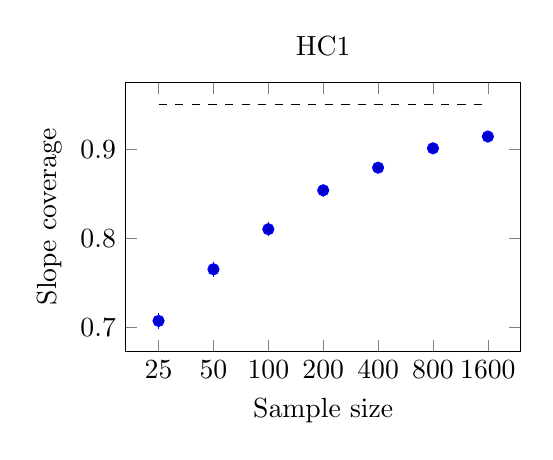
\begin{tikzpicture}
\begin{axis}[width=6.6cm,height=5cm,xlabel={Sample size},ylabel={Slope coverage},title={HC1},xtick={0,1,2,3,4,5,6},xticklabels={{25},{50},{100},{200},{400},{800},{1600}}]
% Interval meaning: Wilson 95% interval for coverage over 10000 trials
\addplot+[no marks,forget plot] coordinates {(0,0.6985055902989736) (0,0.7163350503771957)};
\addplot+[no marks,forget plot] coordinates {(1,0.7569937371114757) (1,0.7736024365533691)};
\addplot+[no marks,forget plot] coordinates {(2,0.8024970904401808) (2,0.8178646001709774)};
\addplot+[no marks,forget plot] coordinates {(3,0.8468413792283328) (3,0.8606868267249023)};
\addplot+[no marks,forget plot] coordinates {(4,0.8727687765377132) (4,0.8855399222982914)};
\addplot+[no marks,forget plot] coordinates {(5,0.8949914473662954) (5,0.906700585940422)};
\addplot+[no marks,forget plot] coordinates {(6,0.9085504560920603) (6,0.9195314396576713)};
\addplot+[only marks,forget plot] coordinates {(0,0.7075) (1,0.7654) (2,0.8103) (3,0.8539) (4,0.8793) (5,0.901) (6,0.9142)};
\addplot[black,dashed,no marks,forget plot] coordinates {(0,0.95) (6,0.95)};
\end{axis}
\end{tikzpicture}
